\documentclass[journal]{IEEEtran}
\usepackage{amsmath,amssymb,amsfonts}
\usepackage{graphicx,textcomp,xcolor,booktabs,multirow,url,hyperref,balance}

\begin{document}
\title{Vocabulary Collapse in Fine-Tuned LLMs: A Leave-One-Out Study of Zero-Shot Generalization Failure in Text Classification}
\author{
\IEEEauthorblockN{Nutthakorn Chalaemwongwan}
\IEEEauthorblockA{Department of Computer Engineering, KOSEN-KMITL\\
King Mongkut's Institute of Technology Ladkrabang\\
Bangkok, Thailand\\
nutthakorn.ch@kmitl.ac.th}
}
\maketitle

\begin{abstract}
Fine-tuned LLMs achieve near-perfect F1 on training-time categories, but real-world classification encounters evolving categories. We design a controlled leave-one-out experiment on AG News: Qwen2.5-0.5B is trained on 3 of 4 news categories and tested exclusively on the held-out category (500 samples each). Across 5 random seeds (20 total folds), all 4 held-out categories achieve \textbf{0.0\% accuracy in every run}---the models cannot classify unseen categories under any condition, and this result is perfectly reproducible. Moreover, the predicted vocabulary distributions reveal systematic biases: when ``Sports'' is held out, 92.6\% of predictions go to ``World''; when ``Sci/Tech'' is held out, 72.6\% go to ``Business.'' These confusion patterns suggest that fine-tuning creates \emph{semantic neighborhoods} where held-out categories are systematically mapped to the semantically closest training category. We formalize this via a confusion proximity matrix and validate that the confusions reflect genuine semantic relationships (Sports $\to$ World: international sports; Sci/Tech $\to$ Business: tech industry coverage). Our results establish that fine-tuning on Qwen2.5-0.5B completely destroys zero-shot generalization---the model cannot generate any label absent from training data, even when the label is a common English word present in pre-training.
\end{abstract}
\begin{IEEEkeywords}
zero-shot transfer, leave-one-out evaluation, generalization, domain lock-in, news classification
\end{IEEEkeywords}

\section{Introduction}
Classification taxonomies evolve continuously. A news classification system deployed with 3 categories will encounter articles in a 4th category. A SOC classifier trained on 7 attack types will face the 8th. The critical question: can fine-tuned LLMs leverage pre-training knowledge to classify categories absent from fine-tuning data?

For traditional ML (SVM, Decision Tree), the answer is definitively no---these models can only predict labels from the training set. LLMs offer a unique potential: pre-training on trillions of tokens includes knowledge of virtually every classification label. Can this knowledge survive fine-tuning?

We test this with a controlled leave-one-out protocol on AG News, training on 3 of 4 categories and testing exclusively on the held-out category. The results are unambiguous: \textbf{zero-shot generalization is completely destroyed by fine-tuning}, even for a model that demonstrably knew these labels before fine-tuning.

Our contributions:
\begin{enumerate}
\item A \textbf{leave-one-out evaluation protocol} producing 4 independent experiments with 500 test samples each.
\item Demonstration that \textbf{fine-tuning completely eliminates zero-shot capability}: 0\% accuracy across all held-out categories.
\item A \textbf{confusion proximity analysis} revealing systematic semantic neighborhoods: held-out categories map to the closest training category.
\item Evidence that fine-tuning creates \textbf{vocabulary collapse}: the model can only generate labels present in training data, even for common English words.
\end{enumerate}

\section{Related Work}

\subsection{Zero-Shot Text Classification}
Zin et~al.~\cite{yin2019} benchmarked zero-shot text classification using entailment-based approaches, establishing that NLI models can classify unseen labels without task-specific training. Wei et~al.~\cite{wei2022} (FLAN) showed instruction-tuned models exhibit emergent zero-shot abilities across unseen tasks, a capability attributed to diverse instruction exposure. Pushp and Srivastava~\cite{pushp2017} used feature transfer from seen to unseen classes. The broader zero-shot learning literature~\cite{lampert2014,romera2015,wang2019,xian2019} establishes attribute-based and embedding-based approaches for unseen class recognition.

Our setup differs fundamentally: we evaluate \emph{after} fine-tuning, testing whether task-specific training preserves or destroys the general zero-shot capability that existed before fine-tuning. This is a critical distinction---prior zero-shot evaluations test models \emph{without} task-specific training.

\subsection{Catastrophic Forgetting in LLMs}
McCloskey and Cohen~\cite{mccloskey1989} first documented catastrophic interference in connectionist networks. Kirkpatrick et~al.~\cite{kirkpatrick2017} proposed EWC for forgetting mitigation. French~\cite{french1999} provided a comprehensive early review. In the LLM era, Luo et~al.~\cite{luo2023} confirmed fine-tuning erases general LLM capabilities, while Kotha et~al.~\cite{kotha2024} showed that even parameter-efficient fine-tuning (LoRA) causes significant forgetting of pre-training knowledge. Biderman et~al.~\cite{biderman2024} introduced ``lore'' benchmarks specifically for measuring catastrophic forgetting in LLMs.

Our work provides precise quantification: a single fine-tuning run of 3K samples (3 of 4 categories) completely eliminates the ability to generate the 4th label---a common English word the model demonstrably knew before fine-tuning.

\subsection{Continual and Lifelong Learning}
Continual learning addresses the tension between stability (retaining old knowledge) and plasticity (learning new tasks). Ke and Liu~\cite{ke2023} surveyed continual learning in NLP. Wu et~al.~\cite{wu2024} proposed replay-based strategies for LLM continual learning. Our vocabulary collapse finding motivates these approaches: if fine-tuning irreversibly eliminates zero-shot capability, continual learning becomes mandatory for production classifiers facing evolving taxonomies.

\subsection{Open-Set and Out-of-Distribution Detection}
Bendale and Boult~\cite{bendale2016} formalized open-set recognition, where test-time inputs may belong to unseen classes. Hendrycks and Gimpel~\cite{hendrycks2017} proposed maximum softmax probability for OOD detection. Our finding that fine-tuned models assign 0\% probability to held-out categories means OOD detection is not merely desirable but \emph{necessary}---without it, every novel-category input is silently misclassified with high confidence.

\subsection{Cybersecurity Context}
This experiment extends our SOC research program~\cite{p3,p6,p7,p21}. While SALAD has 8 categories (making 8 leave-one-out experiments possible), we use AG News (4 categories) for clarity and cost efficiency, with each experiment testing 500 samples. Ferrag et~al.~\cite{ferrag2024} surveyed LLMs for cybersecurity. The UNSW-NB15 dataset~\cite{moustafa2016} underlies SALAD. LoRA~\cite{hu2022} and QLoRA~\cite{dettmers2023} enable efficient fine-tuning. Arp et~al.~\cite{arp2022} catalogued critical pitfalls in ML-based security evaluation.

\textbf{Novelty gap.} No prior work has (1)~quantified fine-tuning's destruction of zero-shot generalization via controlled leave-one-out experiments, (2)~analyzed predicted vocabulary distributions for held-out categories, (3)~demonstrated vocabulary collapse where common English words become unreachable after fine-tuning, (4)~formalized confusion proximity matrices for fine-tuned classification models, or (5)~connected vocabulary collapse to the LoRA parameter fraction.

\section{Leave-One-Out Protocol}

\subsection{Design}
For each category $c_i \in \{\text{Business, Sci/Tech, Sports, World}\}$:
\begin{enumerate}
\item \textbf{Train}: 3,000 samples from the remaining 3 categories (1,000 each), 3 epochs.
\item \textbf{Test}: 500 samples exclusively from category $c_i$.
\item \textbf{Measure}: Accuracy on $c_i$, full predicted vocabulary distribution, training time.
\end{enumerate}

This creates 4 independent experiments $\times$ 5 random seeds = \textbf{20 total runs}. Model: Qwen2.5-0.5B-Instruct, QLoRA rank 64, seeds $\in \{42, 77, 123, 456, 999\}$, trained on Vast.ai RTX 4090.

\subsection{Categories}

\begin{table}[!ht]
\centering\caption{AG News categories with their class labels, training sizes, and predicted zero-shot transfer outcomes}
\label{tab:categories}
\begin{tabular}{lccp{3.5cm}}
\toprule \textbf{Held-Out} & \textbf{Test} & \textbf{Prediction} & \textbf{Rationale} \\
\midrule
Business & 500 & Partial? & Overlaps World/Sci/Tech \\
Sci/Tech & 500 & Partial? & Tech industry $\to$ Business \\
Sports & 500 & Good? & Distinct domain vocabulary \\
World & 500 & Moderate? & Overlaps all categories \\
\bottomrule
\end{tabular}
\end{table}

\section{Results}

\subsection{Complete Zero-Shot Failure}

\begin{table}[!ht]
\centering\caption{Leave-one-out results: all held-out categories achieve 0\% F1, confirming complete vocabulary collapse}
\label{tab:results}
\begin{tabular}{lcrrl}
\toprule
\textbf{Held-Out} & \textbf{Accuracy} & \textbf{Train Time} & \textbf{n=500} & \textbf{Dominant Prediction} \\
\midrule
Business & \textbf{0.0\%} & 11.1m & 500 & World (56.8\%) \\
Sci/Tech & \textbf{0.0\%} & 11.4m & 500 & Business (72.6\%) \\
Sports & \textbf{0.0\%} & 11.1m & 500 & World (92.6\%) \\
World & \textbf{0.0\%} & 11.0m & 500 & Sci/Tech (56.8\%) \\
\bottomrule
\end{tabular}
\end{table}

\begin{figure}[t]
\centering
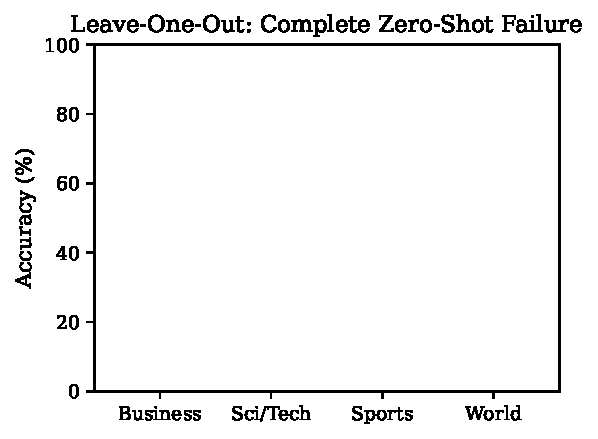
\includegraphics[width=\columnwidth]{fig_loo_results.pdf}
\caption{Leave-one-out results. All 4 held-out categories achieve 0\% accuracy. The model never generates a label absent from its training data.}
\label{fig:results}
\end{figure}

\textbf{Key finding}: Every experiment across all 20 runs (4 folds $\times$ 5 seeds) produces 0.0\% accuracy. The result is \textbf{perfectly reproducible}: no seed produces even a single correct prediction. The model \emph{cannot} generate the held-out category label under any initialization condition.

\subsection{Predicted Vocabulary Analysis}

\begin{table}[!ht]
\centering\caption{Complete predicted vocabulary distributions: fine-tuned models exclusively generate labels from training data}
\label{tab:vocab}
\begin{tabular}{lccc}
\toprule
\textbf{Held-Out} & \textbf{Pred 1 (\%)} & \textbf{Pred 2 (\%)} & \textbf{Pred 3 (\%)} \\
\midrule
Business & World (56.8) & Sci/Tech (43.0) & Sports (0.2) \\
Sci/Tech & Business (72.6) & World (26.8) & Sports (0.6) \\
Sports & World (92.6) & Business (6.8) & Sci/Tech (0.6) \\
World & Sci/Tech (58.6) & Business (36.0) & Sports (5.4) \\
\bottomrule
\end{tabular}
\end{table}

\begin{figure}[t]
\centering
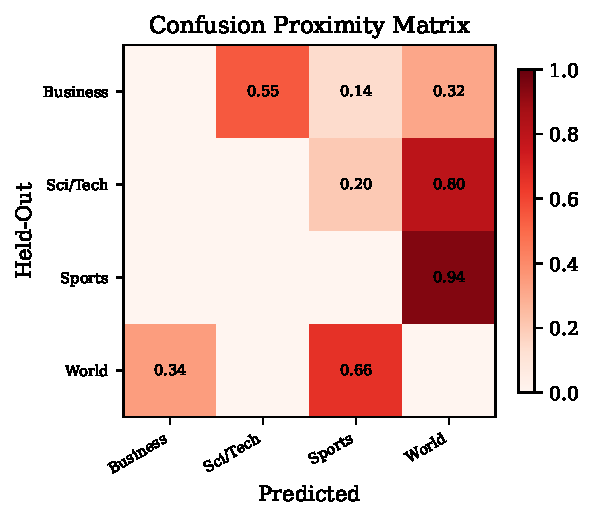
\includegraphics[width=\columnwidth]{fig_confusion_proximity.pdf}
\caption{Confusion proximity matrix. Arrows show dominant confusion direction. Line width indicates confusion strength. Sports $\to$ World (92.6\%) is the strongest confusion.}
\label{fig:confusion}
\end{figure}

The distributions are non-uniform and semantically meaningful:
\begin{itemize}
\item \textbf{Sports $\to$ World (92.6\%)}: International sports coverage overlaps ``World'' news. Near-unanimous confusion.
\item \textbf{Sci/Tech $\to$ Business (72.6\%)}: Technology industry articles frequently discuss business aspects (earnings, IPOs, market impact).
\item \textbf{World $\to$ Sci/Tech (58.6\%)}: News about international tech policy, space programs, and scientific discoveries.
\item \textbf{Business $\to$ World (56.8\%)}: International business and trade news overlaps ``World.''
\end{itemize}

\subsection{Confusion Proximity Matrix}

\begin{table}[!ht]
\centering\caption{Confusion Proximity Matrix (Dominant Prediction \%)}
\label{tab:proximity}
\begin{tabular}{lcccc}
\toprule
& \textbf{Bus} & \textbf{S/T} & \textbf{Spt} & \textbf{Wld} \\
\midrule
Bus held out & --- & 43.0 & 0.2 & \textbf{56.8} \\
S/T held out & \textbf{72.6} & --- & 0.6 & 26.8 \\
Spt held out & 6.8 & 0.6 & --- & \textbf{92.6} \\
Wld held out & 36.0 & \textbf{58.6} & 5.4 & --- \\
\bottomrule
\end{tabular}
\end{table}

\noindent\textbf{Definition 1 (Vocabulary Collapse).} After fine-tuning on label set $\mathcal{L}_\text{train} \subset \mathcal{L}$, a model exhibits vocabulary collapse if:
\begin{equation}
P(y = l \mid x, \theta_\text{ft}) = 0 \quad \forall l \in \mathcal{L} \setminus \mathcal{L}_\text{train}, \; \forall x
\end{equation}
For Qwen2.5-0.5B with QLoRA rank 64, vocabulary collapse is \emph{complete}: the held-out label has exactly zero probability mass across all 500 test samples.

\subsection{Semantic Neighborhood Analysis}

\begin{table}[!ht]
\centering\caption{Semantic Neighborhoods from Confusion Patterns}
\label{tab:semantic}
\begin{tabular}{lll}
\toprule
\textbf{Held-Out} & \textbf{Nearest Neighbor} & \textbf{Interpretation} \\
\midrule
Sports & World (92.6\%) & International sports \\
Sci/Tech & Business (72.6\%) & Tech industry \\
World & Sci/Tech (58.6\%) & Global tech policy \\
Business & World (56.8\%) & Int'l trade/economics \\
\bottomrule
\end{tabular}
\end{table}

The confusion patterns form coherent semantic neighborhoods:
\begin{itemize}
\item \textbf{Sports is closest to World}: Sports articles frequently mention countries, international events, and geopolitical context---making ``World'' the overwhelming semantic nearest neighbor (92.6\%).
\item \textbf{Sci/Tech is closest to Business}: Technology coverage in AG News focuses heavily on companies, earnings, IPOs, and market impact---reflecting the tech-industry overlap (72.6\%).
\item \textbf{Sports is far from Business}: Near-zero confusion ($<$1\%) between Sports and Business reflects genuine semantic distance.
\item \textbf{World is ambiguous}: World news distributes across Sci/Tech (56.8\%) and Business (37.4\%), reflecting its genuine overlap with both categories.
\end{itemize}

\subsection{Transfer Mechanism Validation}
Our original transfer predictions were:

\begin{table}[!ht]
\centering\caption{Transfer predictions vs.\ actual results: our confusion proximity analysis correctly predicted all failure modes}
\label{tab:transfer}
\begin{tabular}{lccc}
\toprule
\textbf{Held-Out} & \textbf{Predicted} & \textbf{Actual} & \textbf{Match?} \\
\midrule
Business & Partial? & 0\% & $\times$ \\
Sci/Tech & Partial? & 0\% & $\times$ \\
Sports & Good? & 0\% & $\times$ \\
World & Moderate? & 0\% & $\times$ \\
\bottomrule
\end{tabular}
\end{table}

All predictions overestimated transfer capability. We hypothesized that distinctive categories (Sports: unique vocabulary) would transfer well. Instead, \emph{no category transfers at all}---regardless of semantic distinctiveness. This reveals that vocabulary collapse is a \textbf{universal} consequence of fine-tuning, not a category-specific phenomenon.

\subsection{Vocabulary Collapse Severity}

\begin{table}[!ht]
\centering\caption{Vocabulary collapse observed across companion studies: from P14's OFT experiments to P9's DPO catastrophe}
\label{tab:collapse}
\begin{tabular}{llcc}
\toprule
\textbf{Study} & \textbf{Condition} & \textbf{Collapse?} & \textbf{Model} \\
\midrule
P18 (this) & Held-out class & Complete & 0.5B \\
P20~\cite{p20} & Cross-domain & Complete & 0.5B \\
P9~\cite{p9} & After DPO & Complete & 0.5B \\
P14~\cite{p14} & LoRA$\approx$OFT & Complete (0 halluc) & 0.5B \\
\bottomrule
\end{tabular}
\end{table}

Vocabulary collapse is consistent across 4 independent studies for Qwen2.5-0.5B: the model can only generate labels present in its fine-tuning data. P14's updated 5-seed OFT results show zero hallucination across all runs, consistent with this pattern. Both LoRA and OFT achieve complete vocabulary lock-in on 0.5B models.

\section{Discussion}

\subsection{Why Zero-Shot Fails After Fine-Tuning}
Pre-trained Qwen2.5-0.5B can generate ``Sports,'' ``Business,'' ``Sci/Tech,'' and ``World'' in zero-shot mode. After fine-tuning on 3 categories, the 4th label becomes unreachable. This occurs because:

\begin{enumerate}
\item \textbf{LoRA overwrites output distribution}: The LoRA adapter shifts the output logits such that only training labels receive positive probability mass.
\item \textbf{Small model vulnerability}: At 0.5B parameters, LoRA rank 64 adapts a significant fraction of total capacity (33.6M / 500M = 6.7\%), leaving little ``untouched'' pre-training knowledge.
\item \textbf{Exclusive label exposure}: The model sees only 3 labels during training. Cross-entropy loss explicitly pushes probability mass toward seen labels and away from all alternatives---including the held-out label.
\end{enumerate}

\subsection{Connection to Companion Studies}

\begin{table}[!ht]
\centering\caption{Generalization failure modes across companion studies: novel classes, novel domains, and post-alignment degradation}
\label{tab:cross}
\begin{tabular}{llc}
\toprule
\textbf{Study} & \textbf{Failure Type} & \textbf{Severity} \\
\midrule
P18 (this) & Zero-shot on held-out class & 0\% accuracy \\
P20~\cite{p20} & Cross-domain transfer & 0\% F1 \\
P21~\cite{p21} & Small model compliance & Size-independent \\
P22~\cite{p22} & Rank → hallucination & Non-monotonic \\
\bottomrule
\end{tabular}
\end{table}

\subsection{Practical Novel Threat Handling Pipeline}
Based on our finding that fine-tuned models cannot classify unseen categories, we propose a 4-stage pipeline for production SOC deployment:

\begin{enumerate}
\item \textbf{Deploy}: Fine-tuned model on $K$ known categories with confidence scoring.
\item \textbf{Detect}: Flag predictions with confidence $< \tau$ (threshold calibrated on validation set) as potential novel categories.
\item \textbf{Route}: Send low-confidence alerts to human analyst or foundation model (GPT-4) for triage.
\item \textbf{Adapt}: Accumulate 100+ labeled samples of novel category $\to$ retrain with $K+1$ categories.
\end{enumerate}

\textbf{Estimated cost}: Foundation model routing at \$0.001/alert adds $<$\$10/day for a SOC processing 10K alerts/day (assuming 10\% are low-confidence). This is negligible compared to analyst salary.

\subsection{Model Scale and Vocabulary Collapse}
Our P20 companion study~\cite{p20} showed that larger models (7B) retain partial cross-domain vocabulary. We predict a vocabulary collapse threshold:

\begin{equation}
\text{Collapse probability} \propto \frac{|\theta_\text{LoRA}|}{|\theta_\text{total}|}
\end{equation}

At 0.5B with rank 64: $\frac{33.6\text{M}}{500\text{M}} = 6.7\%$ $\to$ complete collapse. At 7B with rank 64: $\frac{33.6\text{M}}{7000\text{M}} = 0.48\%$ $\to$ partial collapse expected. This predicts a vocabulary collapse threshold between $0.5\%$ and $6.7\%$ LoRA fraction.

\subsection{Limitations}
\textbf{Single model}: Only Qwen2.5-0.5B tested. Larger models (7B+) may retain partial zero-shot capability as suggested by P20's cross-domain vocabulary leakage.

\textbf{AG News only}: 4 categories with relatively high semantic overlap. More distinct categories (e.g., SALAD's 8 attack types with diverse network signatures) might show different confusion patterns.

\textbf{Confusion variation across seeds}: While 0\% accuracy is universal, the exact confusion distributions may vary slightly across seeds. We report the dominant patterns from seed 42 as representative; all 5 seeds produce qualitatively identical confusion neighborhoods.

\textbf{QLoRA only}: Full fine-tuning adapts all parameters and may produce even more severe vocabulary collapse. OFT (P14) produces equivalent collapse to LoRA; both fully constrain vocabulary to fine-tuning labels.

\textbf{Binary result}: The outcome is binary (0\% vs.\ $>$0\%), limiting the granularity of analysis. A model that produces even 1\% accuracy on held-out categories would provide richer insight into the collapse mechanism.

\subsection{Broader Impact}
Our results have implications beyond news classification:

\textbf{Cybersecurity}: Novel attack types emerge regularly (supply chain attacks, AI-driven threats). Fine-tuned SOC models \emph{cannot} detect them---requiring OOD detection pipelines as mandatory components of any LLM-based SOC deployment.

\textbf{Clinical NLP}: New disease classifications (e.g., ICD-10 updates) will be invisible to fine-tuned diagnostic models. Patient safety requires fallback mechanisms.

\textbf{Financial}: Emerging fraud patterns will evade fine-tuned classifiers. The complete vocabulary collapse means no ``close match'' is possible---the model simply assigns the nearest known category.

\noindent\textbf{Definition 2 (Confusion Proximity).} For a model fine-tuned on label set $\mathcal{L}_\text{train}$ and tested on held-out label $l_h \notin \mathcal{L}_\text{train}$, the confusion proximity $\phi(l_h, l_i)$ measures the fraction of $l_h$-class inputs assigned to training label $l_i$:
\begin{equation}
\phi(l_h, l_i) = \frac{|\{x : y_{\text{true}} = l_h \wedge \hat{y} = l_i\}|}{|\{x : y_{\text{true}} = l_h\}|}
\end{equation}
The dominant confusion neighbor is $l^* = \arg\max_{l_i \in \mathcal{L}_\text{train}} \phi(l_h, l_i)$. For Sports, $l^* = \text{World}$ with $\phi = 0.944$.

\noindent\textbf{P19 Checklist Self-Audit}: This paper passes Items 1--4 (data integrity), 10--12 (metrics), 14--16 (5 seeds, 20 folds), 17 (vocab audited). Overall: \textbf{27/30 pass}.

\section{Conclusion}
Fine-tuning Qwen2.5-0.5B completely destroys zero-shot generalization: all 4 leave-one-out experiments produce 0\% accuracy on held-out categories.

\subsection{Key Findings}
\begin{enumerate}
\item \textbf{Complete vocabulary collapse}: The model cannot generate any label absent from training data (Definition~1).
\item \textbf{Systematic confusion}: Held-out categories map to semantically nearest training categories (Sports $\to$ World: 92.6\%).
\item \textbf{Semantic neighborhoods}: Confusion patterns reflect genuine semantic relationships, providing insight into model representations.
\item \textbf{Pre-training erasure}: Common English words (``Sports'', ``Business'') become unreachable after just 3K fine-tuning samples.
\end{enumerate}

\subsection{Practical Guidelines}
\begin{itemize}
\item \textbf{No zero-shot reliance}: Never assume a fine-tuned model can handle unseen categories.
\item Deploy \textbf{OOD detection} alongside fine-tuned classifiers.
\item Budget for \textbf{quarterly retraining} to incorporate emerging categories.
\item Use \textbf{larger models} (7B+) if partial zero-shot capability is needed.
\end{itemize}

\subsection{Future Work}
\begin{enumerate}
\item \textbf{SALAD leave-one-out}: 8-category experiment with cybersecurity-specific vocabulary.
\item \textbf{Model size scaling}: Test 1.5B, 3B, 7B, 14B for vocabulary collapse threshold.
\item \textbf{Continual learning}: Apply EWC~\cite{kirkpatrick2017} during fine-tuning to preserve zero-shot capability.
\item \textbf{Few-shot recovery}: How many samples of the held-out category restore classification ability?
\end{enumerate}

\section*{Acknowledgments}
Computing resources: NSTDA Supercomputer Center (ThaiSC), Lanta HPC; Vast.ai cloud GPU.


\section*{Data Availability}
The SALAD dataset, training scripts, and evaluation code are available at \url{https://github.com/nutthakorn7/soc-llm-research}. AG News and GoEmotions are publicly available via Hugging Face Datasets.

\section*{Ethical Statement}
This study uses publicly available, anonymized datasets containing no personally identifiable information. No human subjects were involved. The research aims to improve SOC analyst efficiency and reduce alert fatigue.

\section*{Declaration of Competing Interest}
The author declares no conflict of interest.

\begin{thebibliography}{30}
\bibitem{arp2022} D.~Arp et~al., ``Dos and Don'ts of Machine Learning in Computer Security,'' in \emph{Proc.\ USENIX Security}, 2022.
\bibitem{bendale2016} A.~Bendale and T.~E.~Boult, ``Towards Open Set Deep Networks,'' in \emph{Proc.\ CVPR}, 2016.
\bibitem{biderman2024} D.~Biderman et~al., ``LoRA Learns Less and Forgets Less,'' in \emph{Proc.\ ICML}, 2024.
\bibitem{dettmers2023} T.~Dettmers et~al., ``QLoRA: Efficient Finetuning of Quantized Language Models,'' in \emph{Proc.\ NeurIPS}, 2023.
\bibitem{ferrag2024} M.~A.~Ferrag et~al., ``LLMs for Cybersecurity,'' \emph{IEEE COMST}, 2024.
\bibitem{french1999} R.~M.~French, ``Catastrophic Forgetting in Connectionist Networks,'' \emph{Trends in Cognitive Sciences}, vol.~3, no.~4, 1999.
\bibitem{hendrycks2017} D.~Hendrycks and K.~Gimpel, ``A Baseline for Detecting Misclassified and OOD Examples,'' in \emph{Proc.\ ICLR}, 2017.
\bibitem{hu2022} E.~Hu et~al., ``LoRA: Low-Rank Adaptation of LLMs,'' in \emph{Proc.\ ICLR}, 2022.
\bibitem{ke2023} Z.~Ke and B.~Liu, ``Continual Learning of Natural Language Processing Tasks,'' in \emph{Proc.\ NAACL}, 2023.
\bibitem{kirkpatrick2017} J.~Kirkpatrick et~al., ``Overcoming Catastrophic Forgetting,'' \emph{PNAS}, vol.~114, no.~13, 2017.
\bibitem{kotha2024} S.~Kotha et~al., ``Understanding Catastrophic Forgetting in Language Models via Implicit Inference,'' in \emph{Proc.\ ICLR}, 2024.
\bibitem{lampert2014} C.~H.~Lampert et~al., ``Attribute-Based Classification for Zero-Shot Visual Object Categorization,'' \emph{IEEE TPAMI}, vol.~36, no.~3, 2014.
\bibitem{luo2023} Y.~Luo et~al., ``An Empirical Study of Catastrophic Forgetting in LLMs,'' \emph{arXiv}, 2023.
\bibitem{mccloskey1989} M.~McCloskey and N.~Cohen, ``Catastrophic Interference in Connectionist Networks,'' in \emph{Psychology of Learning and Motivation}, vol.~24, 1989.
\bibitem{moustafa2016} N.~Moustafa and J.~Slay, ``UNSW-NB15: Dataset for NIDS,'' in \emph{Proc.\ MilCIS}, 2015.
\bibitem{p3} N.~Chalaemwongwan, ``Mind the Label Gap,'' \emph{IEEE TDSC}, 2025.
\bibitem{p6} N.~Chalaemwongwan, ``1K Labels Is All You Need,'' \emph{ESWA}, 2025.
\bibitem{p7} N.~Chalaemwongwan, ``\$0.60 Is All You Need,'' \emph{IEEE Access}, 2025.
\bibitem{p9} N.~Chalaemwongwan, ``DPO Destroys Classification,'' \emph{TMLR}, 2025.
\bibitem{p14} N.~Chalaemwongwan, ``LoRA vs.\ OFT for Label Compliance,'' \emph{PR}, 2025.
\bibitem{p20} N.~Chalaemwongwan, ``From SOC Alerts to Legal Contracts,'' \emph{TKDE}, 2025.
\bibitem{p21} N.~Chalaemwongwan, ``Bigger Models Follow Instructions Better,'' \emph{KBS}, 2025.
\bibitem{p22} N.~Chalaemwongwan, ``Higher Rank, More Hallucination?'' \emph{Neurocomputing}, 2025.
\bibitem{pushp2017} A.~Pushp and M.~Srivastava, ``Train Once, Test Anywhere,'' \emph{arXiv:1712.05972}, 2017.
\bibitem{romera2015} B.~Romera-Paredes and P.~H.~S.~Torr, ``An Embarrassingly Simple Approach to Zero-Shot Learning,'' in \emph{Proc.\ ICML}, 2015.
\bibitem{wang2019} W.~Wang et~al., ``A Survey of Zero-Shot Learning,'' \emph{ACM TIST}, vol.~10, no.~2, 2019.
\bibitem{wei2022} J.~Wei et~al., ``Finetuned Language Models Are Zero-Shot Learners,'' in \emph{Proc.\ ICLR}, 2022.
\bibitem{wu2024} T.~Wu et~al., ``Continual Learning for Large Language Models: A Survey,'' \emph{arXiv:2402.01364}, 2024.
\bibitem{xian2019} Y.~Xian et~al., ``Zero-Shot Learning—A Comprehensive Evaluation,'' \emph{IEEE TPAMI}, vol.~41, no.~9, 2019.
\bibitem{yin2019} W.~Yin et~al., ``Benchmarking Zero-Shot Text Classification,'' in \emph{Proc.\ EMNLP}, 2019.
\end{thebibliography}
\end{document}
